\section{Background}\label{chap:background}


\paragraph*{}In the complex world of cybersecurity and digital forensics, innovative approaches are crucial for revealing hidden or encrypted information. OpenSSH stands out as a key instrument for ensuring secure communication. The memory snapshots, or heap dumps, of OpenSSH are treasure troves of data. Through graph generation from these dumps, we can uncover the detailed connections between data structures, identified by their malloc headers, and their associated pointers.

\paragraph*{}This research delves deep into the smart embedding of these connections, aiming to use machine learning classifiers to identify structures that contain OpenSSH keys. The journey is not just about representing data through graphs but also about understanding the raw sequences of bytes in the heap dump. Classical techniques like Shannon entropy, \acrfull{bfd}, and bigram frequencies provide foundational knowledge. However, the rapidly evolving domain of deep learning opens up a plethora of avenues. Models such as \acrfull{rnn} \cite{lai_recurrent_2015} (\acrfull{lstm}\cite{hochreiter_long_1997} and \acrfull{gru}\cite{chung_empirical_2014}) and sequence-to-sequence learning \cite{sutskever_sequence_2014} offer unique perspectives on raw byte embedding. Furthermore, the efficacy of convolutional approaches (\acrshort{cnn}), both standalone\cite{lecun_gradient-based_1998} and in conjunction with recurrent networks, for sequence modeling is well-documented \cite{bai_empirical_2018}. Notably, the application of neural networks in file fragment classification, especially with lossless representations, has shown promising results \cite{hiester_file_2018}.Finally, we will dive into transformers and autoencoders.

\paragraph*{}The aim of this background section is to provide a comprehensive overview of graph creation from heap dumps, techniques for raw byte embedding, and their role in identifying OpenSSH key structures. By merging age-old techniques with modern approaches, we strive to highlight the most effective methods for analyzing OpenSSH heap dump.

\subsection{Graph Generation from Heap Dumps}
    \subsubsection{Secure Shell (SSH)}
    
        \paragraph*{}\enquote{The \acrfull{ssh} is designed to enable encrypted communication across potentially unsecured networks, ensuring the confidentiality of data during transmission. Each \acrshort{ssh} session utilizes a specific set of session keys, encompassing six distinct keys:

        \begin{itemize}
            \item \textbf{Key A:} Client-to-server initialization vector (IV)
            \item \textbf{Key B:} Server-to-client initialization vector (IV)
            \item \textbf{Key C:} Client-to-server encryption key (EK)
            \item \textbf{Key D:} Server-to-client encryption key (EK)
            \item \textbf{Key E:} Client-to-server integrity key
            \item \textbf{Key F:} Server-to-client integrity key
        \end{itemize}

        \paragraph*{}To decrypt the encrypted traffic within an \acrshort{ssh} session, knowledge of the IV and EK pair (either Key A with Key C or Key B with Key D) is essential, assuming the presence of passive network monitoring tools. OpenSSH, a prevalent implementation of \acrshort{ssh}, is the primary subject of this research, covering versions from V6\_0P1 to V8\_8P1. OpenSSH incorporates various encryption methodologies, including Advanced Encryption Standard (AES) Cipher Block Chaining (CBC), AES Counter (AES-CTR), and ChaCha20, with IV and EK key lengths varying between 12 and 64 bytes.}
        
        \paragraph*{}This information is derived from the paper titled \citetitle*{fellicious_smartkex_2022} \cite{fellicious_smartkex_2022}.

    \subsubsection{heap dumps of OpenSSH}
        \paragraph*{}\enquote{Heap memory, distinct from local stack memory, is a dynamic memory allocation mechanism. While local stack memory is responsible for storing and deallocating local variables during function calls, heap memory requires explicit memory allocation and deallocation. This is achieved using operators such as \texttt{new} in Java and C++, or \texttt{malloc/calloc} in C.

        \paragraph*{}OpenSSH, which is primarily written in C, employs \texttt{calloc} for memory block allocation. These blocks are designated to store session-related data, including the cryptographic keys. By leveraging this knowledge, one can deduce that if the heap of an active OpenSSH process is dumped at an opportune moment (for instance, during an ongoing SSH session), the resulting heap dump will encompass the \acrshort{ssh} session keys.}

        \paragraph*{}This information is also derived from the paper titled \citetitle*{fellicious_smartkex_2022} \cite{fellicious_smartkex_2022}.

    \subsubsection{Dataset}
        \paragraph{}\enquote{We use SSHKex\cite*{sentanoe_sshkex_2022} as the primary method to extract the \acrshort{ssh} keys from the main memory. In addition, we add two features to SSHKex: automatically dump OpenSSH’s heap and add support for \acrshort{ssh} client monitoring.

        \paragraph{}For this paper, we are using four \acrshort{ssh} scenarios: the client connects to the server and exits immediately, port-forward, secure copy, and \acrshort{ssh} shared connection.
        Two file formats, JSON and RAW, are utilized to store the generated logs. The JSON log file encompasses meta-information, including the encryption name, the virtual memory address of a key, and the key's value in hexadecimal representation (as depicted in Figure~\ref{fig:Background:json}). Conversely, the binary file captures the heap dump of the OpenSSH process (illustrated in Figure~\ref{fig:Background:xxd} using the \texttt{xxd} command).
        \begin{figure}[H]
            \centering
            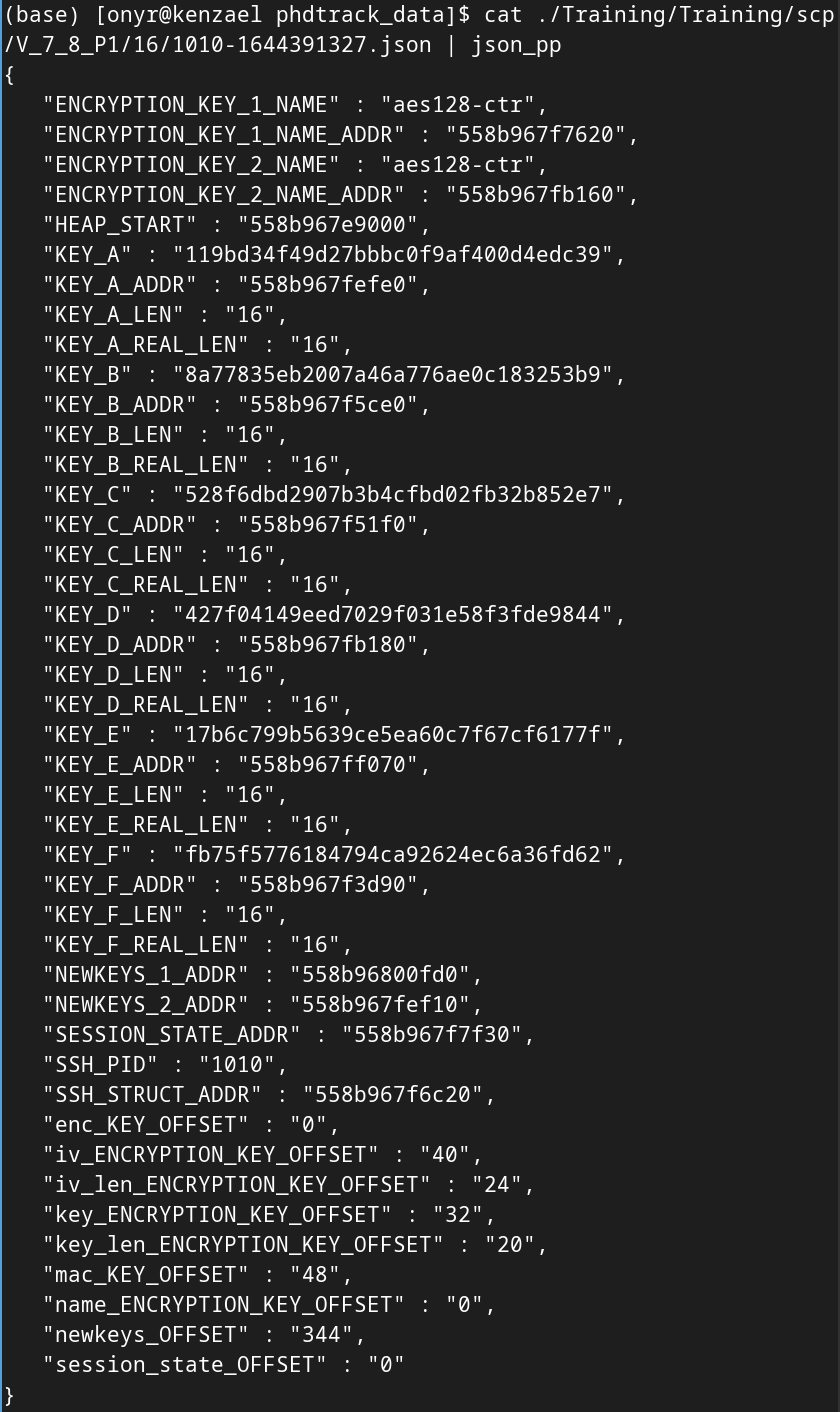
\includegraphics[width=0.6\textwidth]{img/background/json_annotation_for_1010-1644391327.png}
            \caption{Json exemple}
            \label{fig:Background:json}
        \end{figure}

        \begin{figure}[H]
            \centering
            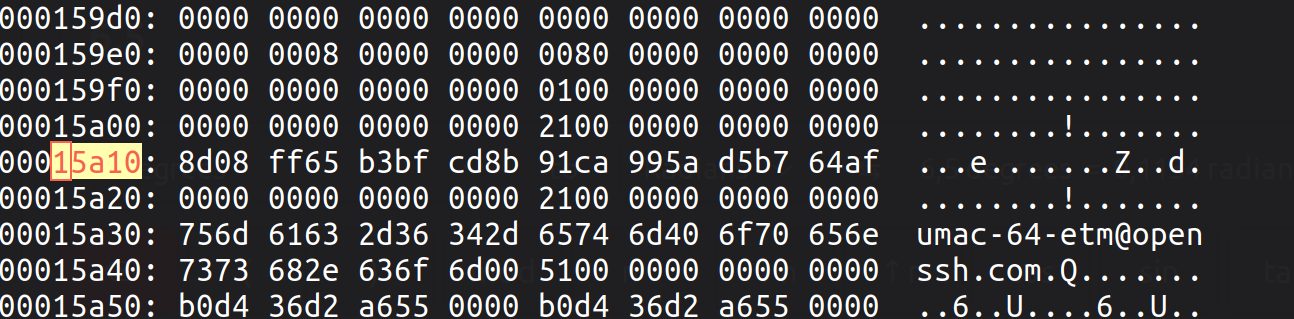
\includegraphics[width=0.6\textwidth]{img/background/xxd.png}
            \caption{Xxd exemple}
            \label{fig:Background:xxd}
        \end{figure}

        \paragraph{}The dataset is structured into two primary directories: \texttt{training} and \texttt{validation}. Each of these directories is further segmented into subdirectories reflecting the specific scenario, such as OpenSSH, port-forwarding, or secure copy (\acrshort{scp}).

        \paragraph{}Subdirectories under OpenSSH or SCP are categorized based on the software version responsible for the memory dump. These directories are further organized by the software version that generated the memory dump. The heaps are then classified based on their key lengths, with each key length possessing its dedicated directory beneath the version directory. These version-specific directories are further divided based on the different key lengths present in a heap.

        \paragraph{}Accompanying every raw memory dump is a JSON file, distinguished by the same alphanumeric sequence, barring the ``-heap'' suffix. This JSON file encapsulates various encryption keys and additional metadata, such as the process ID and the offset of the heap. Consequently, the dataset's utility is not confined to extracting session keys but also extends to identifying crucial data structures harboring sensitive information. The dataset, along with the associated code and tools, is open-sourced. The dataset is accessible via a Zenodo repository\footnote{\url{https://zenodo.org/record/6537904}}. The code can be found in a public GitHub repository\footnote{Link to the GitHub repository}.}
        
        \paragraph{}This data is the same as the data used in the paper titled \citetitle*{fellicious_smartkex_2022} \cite{fellicious_smartkex_2022}.
    
    \subsubsection{Entropy's Role in SSH Key Identification}

        \paragraph{}Encryption keys\cite*{fellicious_smartkex_2022} inherently consist of predominantly random byte sequences. This characteristic stems from the foundational principle of ensuring security through transparency, which guarantees their high entropy. The paper explores the nuances of pinpointing these keys in memory dumps, underscoring the significance of entropy in this endeavor. This particularity can be used to identify the keys in the memory dump.
        
    \subsubsection{Definitions : Structures, Pointers, and the role of malloc headers}
    
        \paragraph{}Through the use of the regular expressions (\acrshort{regex}) \texttt{"[0-9a-f]\{12\}0\{4\}"}, we identified potential \glspl{pointer} within the dump. This heuristic approach acts as a sieve, filtering the extensive data to spotlight possible \gls{pointer} candidates. Nonetheless, it's crucial to understand that while many \glspl{pointer} might be correctly pinpointed, some detected sequences may not be authentic \glspl{pointer}.

        \paragraph{}One notable characteristic of the heap dump is the \textit{malloc header} found at the start of allocated \glspl{structure}. This header, often the initial non-null bytes in a series, signifies the size of the following \gls{structure}. By sequentially reading the heap dump and identifying these headers, it becomes feasible to determine the dimensions and limits of every allocated \gls{structure}, thereby methodically dividing the heap dump into distinct \glspl{structure}.
        
\subsection{Traditional Statistical Embedding}

    \paragraph{}Within the domain of machine learning, how data is represented significantly impacts the performance of models. Even though traditional statistical embedding techniques have been around before many contemporary methods, they continue to be vital in readying data for machine learning endeavors. Rooted in statistical foundations, these techniques provide a methodical approach to transform raw data into concise and meaningful forms. In this subsection, we'll delve into the nuances of entropy and its role in byte sequence embedding, \acrfull{bfd}, and also highlight other classical statistical embedding methods pivotal in data representation for machine learning.
        
    \subsubsection{Entropy and its application in byte sequence embedding}
        \paragraph{}Entropy, a fundamental concept in information theory, quantifies the amount of uncertainty or randomness associated with a set of data. Introduced by Claude Shannon in his groundbreaking work \cite{shannon_mathematical_1948}, entropy serves as a measure of the average information content one can expect to gain from observing a random variable's value.

        \paragraph{}Mathematically, the entropy \(H(X)\) of a discrete random variable \(X\) with possible values \newline \(\{x_1, x_2, \ldots, x_n\}\) and probability mass function \(P(X)\) is given by:
        \begin{align}
            H(X) &= -\sum_{i=1}^{n} P(x_i) \log_2 P(x_i)
            \label{eq:shannon_entropy}
        \end{align}

        \paragraph{}Within the scope of identifying SSH keys, the significance of entropy cannot be understated. Byte sequences exhibiting high entropy typically reflect a multifaceted and varied informational content, traits that are synonymous with encryption keys, especially those in SSH. Sequences with pronounced entropy are often prime contenders for SSH keys due to their inherent randomness and lack of predictability, mirroring the attributes of robust security keys.

        \paragraph{}Fundamentally, entropy acts as a quantitative tool to evaluate the depth of information within data. When applied to SSH, it suggests that data sequences with elevated entropy levels have a heightened probability of correlating with secure keys. This positions entropy as an essential instrument for pinpointing and authenticating SSH keys.
    \subsubsection{Byte Frequency Distribution (BFD)}
        \paragraph{}In the complex world of raw byte embedding, \acrfull{bfd} and n-gram embedding stand out as essential methods, each bringing unique benefits to data representation. \acrshort{bfd} zeroes in on the distribution of individual byte values in a raw byte sequence. Analyzing these distributions allows for the identification of patterns that reflect the inherent nature of the data. This embedding technique becomes particularly relevant when assessing the randomness or structure of byte sequences, such as when detecting encrypted data or pinpointing specific file signatures.

        \paragraph{}On the other hand, n-gram embedding dives deeper into raw byte sequences. Instead of focusing solely on individual bytes, it captures patterns formed by sequences of 'n' consecutive bytes. This approach garners a wider range of contextual information from the raw byte data. For example, a trigram (3-gram) examines patterns formed by three sequential bytes, providing a richer representation than single byte values. Yet, a challenge with n-gram embedding is the potential for the output vector size to grow exponentially as 'n' increases, posing computational and storage issues, especially in real-time scenarios.
        
        \paragraph{}In the realm of raw byte embedding, both \acrshort{bfd} and n-gram techniques offer invaluable perspectives. While \acrshort{bfd} establishes a base representation centered on individual byte frequencies, n-gram embedding enhances it by spotlighting the complex relationships and patterns among consecutive bytes. Together, they form a robust arsenal for representing and analyzing raw byte data in a variety of applications.
    \subsubsection{Other traditional statistical embedding techniques}
        \paragraph{Mean Byte Value}The Mean Byte Value represents the average value of all bytes in a given sequence. It provides an insight into the central tendency of the byte values in the sequence. Mathematically, for a byte sequence \( B \) of length \( n \):
        \begin{equation}
        \text{Mean Byte Value} = \frac{1}{n} \sum_{i=1}^{n} B_i
        \label{eq:mean_byte_value}
        \end{equation}

        \paragraph{Mean Absolute Deviation (MAD)}MAD measures the average distance of each byte value from the mean, providing a sense of the dispersion or spread of the byte values around the mean. It is given by:
        \begin{equation}
        \text{MAD} = \frac{1}{n} \sum_{i=1}^{n} |B_i - \text{Mean Byte Value}|
        \label{eq:mad}
        \end{equation}

        \paragraph{Standard Deviation}Standard Deviation quantifies the amount of variation or dispersion in the byte sequence. A higher value indicates greater variability in the byte values. It is defined as:
        \begin{equation}
        \text{Standard Deviation} = \sqrt{\frac{1}{n} \sum_{i=1}^{n} (B_i - \text{Mean Byte Value})^2}
        \label{eq:standard_deviation}
        \end{equation}

        \paragraph{Skewness}Skewness\cite{wheeler_problems_2011} measures the asymmetry of the distribution of byte values around the mean. A positive value indicates a distribution that is skewed to the right, while a negative value indicates a distribution skewed to the left. It provides insights into the shape of the distribution of byte values. The Fisher’s skewness\cite{cain_univariate_2017} is :
        \begin{equation}
        \text{Skewness} = \frac{n}{(n-1)(n-2)} \sum_{i=1}^{n} \left( \frac{B_i - \text{Mean Byte Value}}{\text{Standard Deviation}} \right)^3
        \label{eq:skewness}
        \end{equation}

        \paragraph{Kurtosis}Kurtosis\cite{wheeler_problems_2011} measures the "tailedness" of the distribution of byte values. A higher kurtosis value indicates a distribution with heavier tails, while a lower value indicates lighter tails. It provides insights into the extremities of the distribution. The Fisher’s kurtosis\cite{cain_univariate_2017} is :
        \begin{equation}
        \text{Kurtosis} = \frac{n(n+1)}{(n-1)(n-2)(n-3)} \sum_{i=1}^{n} \left( \frac{B_i - \text{Mean Byte Value}}{\text{Standard Deviation}} \right)^4 - \frac{3(n-1)^2}{(n-2)(n-3)}
        \label{eq:kurtosis}
        \end{equation}

        \paragraph{n-gram on Bits}When applying n-gram techniques to bits instead of bytes, we focus on sequences of 'n' consecutive bits. For example, a 2-gram on bits would consider patterns formed by two consecutive bits, resulting in four possible combinations: 00, 01, 10, and 11. This approach significantly reduces the size of the output vector compared to byte-based n-grams. By focusing on bits, we can capture more granular patterns in the data while benefiting from a more compact representation, which is computationally efficient and requires less storage.

\subsection{Deep Learning Models for Raw Byte Embedding}

    \paragraph{}In the area of data representation, deep learning is great for understanding raw byte sequences. Just like these models are good at understanding text, they're also good at understanding raw bytes. They can learn and show sequences on their own, which is really helpful for both text and raw bytes. In this section, we'll look at different deep learning models and how they work with raw byte embedding.

    \paragraph{}We'll start with \acrfull{rnn}. Just like they're good with word sequences in text, \acrfull{rnn} are also good with raw byte sequences. Then, we'll look at \acrfull{cnn}, which can find patterns in raw bytes, just like they find patterns in text. After that, we'll talk about Autoencoders, which can learn in a special way. To finish this section, we'll discuss Transformers. They're good at understanding data over a long time, similar to how they understand text.

    \subsubsection{RNNs : Understanding sequence data}
        \paragraph{}\acrfull{rnn} are great tools for text classification. They're good at understanding the deeper meanings in text. Unlike older models that use hand-made features, \acrshort{rnn} can learn and show sequences on their own. This makes them really useful for tasks that deal with sequences. When we think about embedding raw bytes, \acrshort{rnn}'s skill in understanding sequences is similar to how they handle word sequences in text. Here is a list of different \acrshort{rnn} models and their advantages and disadvantages.

        \paragraph{\acrfull{rcnn} for Text Classification\cite{lai_recurrent_2015}:} The \acrshort{rcnn} model, as discussed in the paper by Lai et al., is designed specifically for text classification. Unlike traditional models, \acrshort{rcnn} do not rely on handcrafted features. Instead, they employ a recurrent structure to capture contextual information about words. This approach is believed to introduce considerably less noise compared to traditional window-based neural networks. The model's bidirectional structure ensures that both preceding and succeeding contexts of a word are considered, enhancing its understanding of the word's semantics.

        \begin{itemize}
            \item \textbf{Advantages:} 
            \begin{itemize}
                \item No need for handcrafted features.
                \item Captures richer contextual information.
                \item less noisy.
            \end{itemize}
            \item \textbf{Disadvantages:} 
            \begin{itemize}
                \item Complexity due to bidirectional structure.
                \item Might require more computational resources.
            \end{itemize}; 
        \end{itemize}

        \paragraph{\acrfull{lstm}\cite{hochreiter_long_1997}:}The \acrshort{lstm}, introduced by Hochreiter and Schmidhuber, is a specialized form of \acrshort{rnn} designed to combat the vanishing gradient problem inherent in traditional \acrshort{rnn}. The vanishing gradient problem arises when gradients of the loss function, which are used to update the network's weights, become too small for effective learning. This typically happens in deep networks or when processing long sequences, causing the earlier layers or time steps to receive minimal updates. As a result, traditional \acrshort{rnn} struggle to learn long-term dependencies in the data.

        \paragraph{}\acrshort{lstm} address this issue with their unique cell state and gating mechanisms. The cell state acts as a "conveyor belt" that can carry information across long sequences with minimal changes, ensuring that long-term dependencies are captured. The gating mechanisms, namely the input, forget, and output gates, regulate the flow of information into, out of, and within the cell. This design allows LSTMs to selectively remember or forget information, making them adept at learning and retaining long-term dependencies in sequences.

        \begin{itemize}
            \item \textbf{Advantages:}
            \begin{itemize}
                \item Efficiently learns long-term dependencies; overcomes the vanishing gradient problem inherent in traditional \acrshort{rnn}.
                \item Often achieves faster and more stable learning.
            \end{itemize}
            \item \textbf{Disadvantages:}
            \begin{itemize}
                \item More complex architecture compared to basic \acrshort{rnn} and even \acrshort{gru}.
                \item Can be computationally intensive due to the multiple gating mechanisms.
            \end{itemize}
        \end{itemize}

        \paragraph{\acrfull{gru}\cite{chung_empirical_2014}:} \acrshort{gru} are a variant of \acrshort{rnn} that aim to capture long-term dependencies without the complexity of \acrshort{lstm}. They use a gating mechanism to control the flow of information, making them efficient in sequence modeling tasks.

        \begin{itemize}
            \item \textbf{Advantages:} 
            \begin{itemize}
                \item Simplified structure compared to \acrshort{lstm}.
                \item Efficient in capturing long-term dependencies.
                \item Sometimes outperforms \acrshort{lstm}.
            \end{itemize}
            \item \textbf{Disadvantages:} 
            \begin{itemize}
                \item Still more complex than traditional \acrshort{rnn}.
                \item Might not always outperform \acrshort{lstm} in all tasks.
            \end{itemize}
        \end{itemize}
        

        \paragraph{}To sum it up, \acrshort{rnn} are good at understanding sequences and context. This makes them a good choice for embedding raw bytes. Just like they understand words based on the words around them, \acrshort{rnn} can find patterns in raw byte sequences, giving us a better understanding of the data.
    \subsubsection{CNNs : Pattern detection in raw bytes}
        \paragraph{}\acrfull{cnn}\cite{lecun_gradient-based_1998} are a specialized category of deep learning models adept at identifying patterns. Originally designed for visual data, their prowess extends to tasks like image and document recognition. Drawing inspiration from the human visual cortex's biological processes, \acrshort{cnn} are architected to autonomously and adaptively discern spatial feature hierarchies from inputs. This becomes particularly relevant when considering raw byte embedding, where the goal is to detect patterns in sequences of bytes. The CNN architecture boasts convolutional layers that perform operations on input data to capture localized patterns, and pooling layers that condense spatial dimensions while preserving crucial information. This layered approach enables \acrshort{cnn} to detect intricate patterns by progressively building on simpler foundational patterns. When applied to byte sequences or document recognition, \acrshort{cnn} excel, showcasing remarkable efficacy, especially in tasks like identifying patterns within raw byte sequences or recognizing handwritten content.

        \paragraph{}When tailored to \acrshort{cnn}, the \acrfull{seq2seq}\cite{gehring_convolutional_2017} approach emerges as a potent tool for transforming raw byte sequences into meaningful embeddings. The encoder segment of the \acrshort{seq2seq} model is central to this transformation. It delves into the byte sequence, discerning intricate patterns and nuances, and distills this rich information into a concise context vector or embedding. This condensed representation captures the core essence of the byte sequence, positioning it as a valuable input for subsequent tasks, such as classification models.

        \paragraph{}At the heart of the encoder lie the convolutional layers, skilled in pinpointing specific patterns within the byte sequence. Whether it's unique byte combinations or indicative n-grams, these layers are primed to detect them. As they traverse the raw byte sequence, they employ specialized filters, honed to recognize these specific patterns. As the data flows through the encoder's layers, these identified patterns are synthesized and refined, culminating in a comprehensive embedding of the sequence.
        
        \paragraph{}Having explored the capabilities of CNNs and their sequence-to-sequence adaptations in raw byte embedding, it's pertinent to shift our focus to another transformative architecture in deep learning: autoencoders. 
    \subsubsection{Autoencoders}
        \paragraph{}Autoencoders\cite{hinton_reducing_2006} are neural network designs specifically crafted for data compression and its subsequent reconstruction. They revolve around two main pillars: the encoder and the decoder. The encoder's role is to transform the input data into a tighter format, often labeled as the "latent space" or "embedding." This compacted version holds the essence and primary features of the input, proving invaluable for tasks that require a refined representation of raw byte sequences.

        \paragraph{}A distinguishing trait of the encoder within an autoencoder is its inherent ability to identify and encapsulate the most crucial elements of the input data, all without explicit guidance. When we talk about raw bytes, this means the encoder's adeptness at detecting intrinsic patterns and relationships in the byte sequences, leading to a comprehensive and insightful embedding.
        
        \paragraph{}Yet, a significant challenge with traditional autoencoders, even those adopting a \textit{sequence-to-sequence} pattern, is their constraint in managing inputs of varying sizes. Constructed with a set input size, they face difficulties when presented with sequences of diverse lengths, like raw byte sequences. This limitation can be problematic, especially when byte sequences differ considerably in length and may be not suitable for raw bytes embedding.
    \subsubsection{Transformers}
\subsection{Graph Embedding Methods}
    Wait Onyr

\subsection{Conclusion and Transition to the Next Section}
